\section{Introduction}

%Outline
%
%\begin{enumerate}
%  \item purpose, motivation
%  \begin{itemize}
%    \item online processing of data
%    \item monitoring of trace properties, specifically execution traces of programs
%    \item Functional reactive programming as related concept
%  \end{itemize}
%  \item What you describe with a \tessla specification
%  \begin{itemize}    
%    \item input, output streams
%    \item application of functions, composition of function
%    \item 
%  \end{itemize}
%  \item Modelling data in terms of streams
%  \begin{itemize}
%    \item timing model ($ℝ$,$ℕ$,$ℚ$,…), restrictions to streams with discrete set of time stamps (event streams) or peace-wise constant streams (continuous stream)
%    \item continuous streams and event streams    
%   \end{itemize}
%   \item Functions on streams and desired properties (in general)
%   \begin{itemize}
%     \item small examples
%     \item causality, statefulness, time invariance 
%     \item (composition lemmata)
%   \end{itemize}
%   \item \tessla syntax
%   \begin{itemize}
%      \item base grammar with functions and type annotations
%      \item syntactical extensions: infix operators, named arguments, the “on”
%   \end{itemize}
%   \item Types
%   \begin{itemize}
%     \item Generic types
%     \item Coercion 
%   \end{itemize}
%   \item Functional semantics of operators, small examples
%   \item Larger example/case study
%   \begin{itemize}
%     \item producer/consumer, ring buffer, …
%   \end{itemize}
%   
%   
%\end{enumerate}


Purpose of \tessla.

\begin{itemize}
  \item analysis of trace data
  \item specification of failure patterns, correctness properties, transformations
  \item intuitive, pragmatic means of formulation 
\end{itemize}

Purpose of this document.
\begin{itemize}
  \item Motivate and describe the language
  \item reference
  \item case study and examples from the targeted application area
  \item description of how to integrate runtime verification methodology based on tessla and its implementation into the development process
\end{itemize}

Approach
  \begin{itemize}
    \item online processing of data
    \item monitoring of trace properties, specifically execution traces of programs
    \item Functional reactive programming as related concept
  \end{itemize}

\subsection{What you describe with a \tessla specification}

\tessla is conceptually based on streams as a model for data processing and data analysis. 
The data to be analysed is considered as input streams and a \tessla specification essentially describes a set of output streams and how they can be derived from the input.
To this end, new streams can be defined by applying some function to existing ones.
For example, given an input stream of integral values, a \tessla specification could describe the stream that consecutively provides the sum of all previous input values.
This is achieved by applying a corresponding function to the input stream and thereby defining a new output stream.

\subsection{Stream Model}
\label{sec:streams}

\begin{figure}
  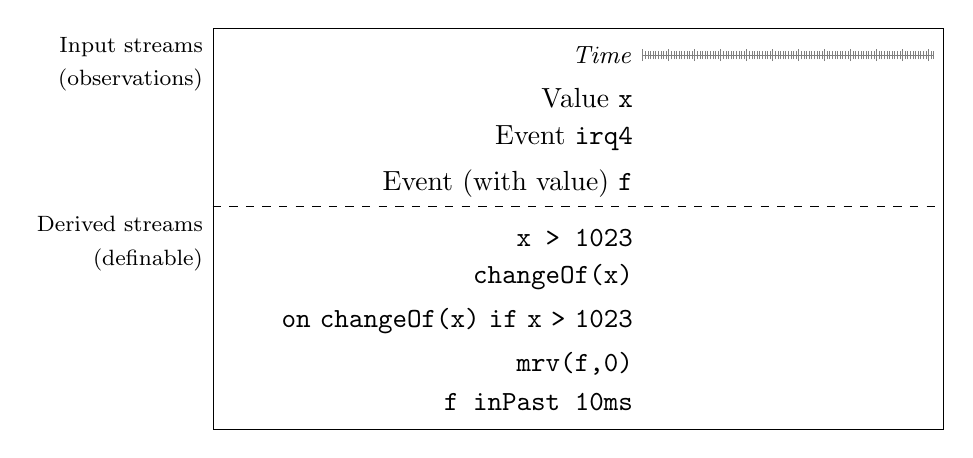
\begin{tikzpicture}

\matrix[column sep = 0.5em, draw] (m) {
  \node[anchor = east] {\small \textit{\textrm{Time}}}; \& \draw[help lines] (0,-0.05) grid[xstep=0.033] (3.7,0.05);
     \draw[gray] (0,-0.075) grid[xstep=0.33] (3.7,0.075); \\[0.5ex]
  \node[anchor = east] (m-1-2) {Value \texttt{x}}; \& \timing[name=m-2-2] at (0,-0.15) {2D{998}N(x1)2D{42}3D{2012}3D{1280}DD{10}DD{1404}};\\
%
  \node[anchor = east] (m-1-3) {Event \texttt{irq4}}; 
    \& \timing[name=m-2-3] at (0,-0.15) {ZZZ \n{} Z \n{} ZZZZ \n{} ZZ \n{} ZZZ \n{} Z}; \\ 
%
  \node[anchor = east] (end-inputs) {Event (with value) \texttt{f}}; 
    \& \timing[name = end-inputs-2] at (0,-0.15) {Z \n{17} ZZZZZZZ \n{98} Z \n{0} ZZZZ \n{23} Z}; \\[0.5em]
%
     \node[anchor = east] (m-1-5) {\texttt{x > 1023}}; 
  \& \timing[name=m-2-5] at (0,-0.15) {4L 6H 2L 2H}; \\ 
% 
     \node[anchor = east] (m-1-6) {\texttt{changeOf(x)}}; 
  \& \timing[name=m-2-6] at (0,-0.15) {2Z \n{} 2Z \n{} 3Z \n{} 3Z \n{} 2Z \n{} 2Z}; \\ 
% 
     \node[anchor = east, text width = 14.5em, align = right] (m-1-7) {
          \texttt{\textbf{on} changeOf(x) \textbf{if} x > 1023}}; 
  \& \timing[name=m-2-7] at (0,-0.15) {4Z \n{} 3Z \n{} 3Z 2Z \n{} 2Z}; \\ 
%  
     \node[anchor = east] (m-1-8) {\texttt{mrv(f,0)}}; 
  \& \timing[name=m-2-8] at (0,-0.15) {D{0} 7D{17} D{98} 4D{0} D{23}}; \\
% 
     \node[anchor = east] (m-1-9) {\texttt{f inPast 10ms}};
  \& \timing[name=m-2-9] at (0,-0.15) {L 2H 5L 3H 2L H}; \\
%
 };
 
\path[draw, dashed] (m.west|-end-inputs.south) edge (m.east|-end-inputs.south);

\path (m.north west) node[anchor = north east, align = right] 
{\footnotesize{Input streams} \\ \footnotesize{(observations)}};

\path (m.west|-end-inputs.south) node[anchor = north east, align = right] {
  \footnotesize{Derived streams} \\ \footnotesize{(definable)}};

\end{tikzpicture}

  \caption{Example streams.\label{fig:streams}} 
\end{figure}

The streams used in \tessla specifications model the essential aspects found in computer programs, namely values (e.g., the value of a program variable), events (e.g., the call of a specific function) and time, both, in a qualitative (ordering) and quantitative (duration) sense.

The timing model is based on time stamps $t∈𝕋$ where we assume $𝕋$ to be isomorphic to the real numbers $ℝ$.\footnote{Notice that we deliberately choose \emph{the continuum} as a model of real time as is common in philosophy, physics and engineering. For our purposes of specifying timing property, however, also a weaker notion of density would clearly suffice, such as the rational numbers $ℚ$.}
Although on the technical level time is mostly quantised in actual systems, real time is a common and intuitive model.
In fact, neither specification nor evaluation based on single steps of, e.g., the a CPU core are reasonable. 
Time is therefore handled, formally and technically, in terms of intervals.
In the following, we make the notion of streams precise that provide the semantic basis of the language.
We use $𝕋$ to denote the time domain to make an explicit distinction between time stamps and, e.g., real values.
This avoids confusion and inconsistencies since the representation of time values is implementation dependent.
For example, the values may be scaled according to the processing clock speed and therefore adding or comparing a value $t∈𝕋$ with some real value $r∈ℝ$ is not well defined unless considering a specific execution platform with fixed parameters.
However, we use common operators and symbols to work with time stamps, such as $+$ (addition), $≤$ (ordering) and $0$ (neutral element of addition), that are defined as expected.

We consider two types of streams.
Values, e.g., of a program variable or stored at some specific memory address, might change over time but can be assumed to always be present.
They are represented by continuous streams that we call \emph{signals}. \todo{adde preliminary definitions somewhere, e.g., appendix: piece-wise constant function, segments, intervals, left/right-closed, change points}

\begin{definition}[Signals]
  Let $D$ be a set of data values. 
  A \emph{signal of type $D$} is a function $σ: 𝕋_{≥0} → D$ such that
  \begin{itemize}
    \item $σ$ is piece-wise constant,
    \item every segment $I∈\mathsf{seg}(σ)$ is left-closed\footnote{
          A \emph{segment} of a piece-wise constant function $σ: 𝕋_{≥0} → D$ is a maximal interval $I⊂𝕋$ with constant value $v∈D$, i.e., $∀_{t∈I}:σ(t)=v$.} and
    \item the set of change points $Δ(σ) := {\min I|I∈\mathsf{seg}(σ)}$ is discrete\footnote{A subset $M$ of $𝕋$ is \emph{discrete} if it does not contain bounded infinite subsets.}.
  \end{itemize}
  The set of all signals $σ: 𝕋_{≥0} → D$ is denoted $𝓢_D$.
\end{definition}

Apart from values that are conveniently modeled to be continuously available, discrete \emph{events}, like function calls, are of interest.
These are modelled by the second type of streams \emph{event streams} that provide values (events) only at specific points in time wheras no information about the time between two consecutive events is available.

\begin{definition}[Event streams]
  For a set $D$ of data values an \emph{event stream of type $D$} is a partial function $η: 𝕋_{≥0} ⇁ D$ such that the domain of definition, called the set of \emph{event points} $E(η) := \{t∈𝕋|η(t)∈D \text{ defined}\}$, is discrete.
%
  The set of all event streams $η: 𝕋_{≥0} ⇁D$ is denoted $𝓔_D$.
\end{definition}

For convenience we may write $η(t) = ⊥$ to denote that $η$ is not defined at time point $t∈𝕋∖ E(η)$.
To model streams of events that do not carry a value we use a designated type \texttt{Unit}.
Formally, we let $\mathtt{Unit}={⊤}$ be a set with one designated element $⊤$.

The discreteness condition reflects the property of actual systems that time stamps cannot converge because only a bounded number of events can happen within a fixed time period.

In addition to the definition in terms of partial functions, an event stream $η∈𝓔_D$ can be naturally represented as a (possibly infinite) sequence $s_η=(t_0,η(t_0))(t_1,η(t_1))…∈(E(η)×D)^∞$ ordered by time ($t_i<t_{i+1}$ for $0≤i<|s_η|$) and containing all event points (i.e, ${t|(t,v) \text{ occurs on } s_η}= E(η)$).

\subsection{Defining Streams}

\tessla allows for defining streams through function applications.
Such functions can be applied to signal and event streams, as well as constant values.
For example, addition of two (value) streams can be defined as element-wise addition of the values of two signals \texttt{s1} and \texttt{s2}:
\begin{lstlisting}[language=tessla]
  define sum := add(in1, in2)
\end{lstlisting}
Here, $\mathtt{add}: 𝓢_ℕ × 𝓢_ℕ → 𝓢_ℕ$ is a function that maps a pair of signals $\mathtt{in1},\mathtt{in2}∈𝓢_ℕ$ with data domain $ℕ$ to the signal representing their sum at every point in time, i.e.,  $\mathtt{sum}(t) = \mathtt{add}(\mathtt{in1}, \mathtt{in2})(t) = \mathtt{in1}(t) + \mathtt{in2}(t)$ for any time point $t∈𝕋$.

The specification above hence describes a rather simple transformation of two input streams into one output stream.

Regarding evaluation it is reasonable to restrict the functions on streams that can be used in \tessla, depending on their application context.

\begin{definition}[Causality, state, time invariance]
Let $A,B$ be sets of signals or event streams.
A function $f: A → B$ is considered to \emph{respect weak causality} if there is a constant $k∈𝕋$ such that $f(σ)(t)$ is independent of the values $σ(t')$ for $t'>t+k$:
for all $t∈𝕋$ and all $σ,σ'∈A$ we require that $f(σ)(t) = f(σ')(t)$ if $σ(t')=σ'(t')$ for all $t'<t+k$.

The function $f$ is called \emph{stateless} if for all $t∈𝕋$ and all $σ,σ'∈A$ we have $f(σ)(t) = f(σ')(t)$ if $σ(t) = σ'(t)$.

A stateless function $f$ is called \emph{time invariant} if $σ(t) = σ(t')$ implies that $f(σ)(t) = f(σ)(t')$ for all $σ∈A$ and all $t∈𝕋_{≥0}$.
\end{definition}


\idea[inline]{
Example: Detecting a delayed action

Assume the control of a device is supposed to react on an input signal within a specific time bound of 10 microseconds.
The control program receives a signal when the function \texttt{rcv()} is called, needs to process the data and react by calling a function \texttt{react()}.
Given means to observe function calls during the execution of the program\footnote{We will discuss observation approaches in Section~\ref{sec:observation}.} a \tessla specification can be used to formulate the timing constraint.
The calls to \texttt{rcv()} and \texttt{react()} can be considered as input event streams \texttt{rcv} and \texttt{react}.

}